A classical problem in quantum mechanics models a particle moving in
an infinite square well, subject to an infinite potential at a point.
The result is a Schr\"odinger operator posed on $C^2_D[0,1]$ of the form
\[ L u = -u'' + \delta_{1/2} u,\]
where $\delta_{1/2}$ is a ``delta function'' centered at the location of
the infinite potential, $x=1/2$.  A beautiful theory supports these
exotic functions (more properly called \emph{distributions}).  
For this problem,
you need only know the following fact: for any function $g\in C[0,1]$,
\[ \int_0^1 \delta_{1/2}(x) g(x) \ d x = g(1/2).\]

The equation $Lu = f$ has the equivalent weak form
\[ a(u, w) = (f,w) \qquad \mbox{for all $w\in V = C^2_D[0,1]$},\]
where
\[ \kern6pt a(u,w) = \int_0^1 \Big(u'(x) w'(x) + \delta_{1/2}(x) u(x) w(x)\Big)\, d x.\]

\vspace*{1em}
We wish to use the Galerkin method to approximate solutions to $Lu = f$
from the finite dimensional subspace
$V_N = {\rm span}\{\phi_1, \ldots, \phi_N\}$.
Use as basis vectors the eigenfunctions from the problem
without the potential at $x=1/2$:
\[ \phi_k(x) = \sqrt{2} \sin(k \pi x).\]

\vspace*{1em}

\begin{enumerate}
\item Compute a general formula for $a(\phi_j, \phi_k)$.

\vspace*{1em}
\item Write out (by hand) the stiffness matrix for $N=5$.

\vspace*{1em}
\item Write down a general formula for the entries in the load vector, $(f,\phi_k)$,
      when $f(x) = 1$.\\  (You may use formulas from prior homework.)

\vspace*{1em}
\item Plot your approximate solutions to $-u''(x) + \delta_{1/2}(x) u(x) = 1$
      for $N=5$ and $N=35$.
\end{enumerate}


\ifthenelse{\boolean{showsols}}{\begin{solution}
\begin{enumerate}
\item Compute
\begin{eqnarray*}
   a(\phi_j,\phi_k) &=& \int_0^1 \big(\phi'_j(x)\phi'_k(x)+\delta_{1/2}(x) \phi_j(x)\phi_k(x)\big)\,dx \\[0.5em]
                    &=& 2 k j \pi^2 \int_0^1 \cos(j \pi x)\cos(k \phi x)\, dx 
                         + 2 \int_0^1 \delta_{1/2}(x) \sin(j\pi x)\sin(k\pi x) \\[.5em]
                    &=& 2 k j \pi^2 \int_0^1 \cos(j \pi x)\cos(k \phi x)\, dx 
                         + 2 \sin(j\pi/2)\sin(k\pi/2).
\end{eqnarray*}
The integral in this last expression is $1/2$ when $j=k$, and zero otherwise.
The second term will be zero if either $j$ or $k$ is even (since in that case one of 
the sine terms must be zero).  If both $j$ and $k$ are odd, this term will be nonzero,
$\pm 2$.
In general, we can write
\[ a(\phi_j,\phi_k) 
     = \left\{\begin{array}{cc}
           j^2 \pi^2 +2\sin^2(j\pi/2), & \mbox{if $j=k$};\\[.5em]
           2\sin(j\pi/2)\sin(k\pi/2),  & \mbox{otherwise}.
       \end{array}\right.\]

[\textbf{GRADERS}: the amount that students simplify $a(\phi_j,\phi_k)$ will vary.
The ultimate solution need not take the precise form that we have given above,
but it should be simplified beyond just writing down the definition of $a(\phi_j,\phi_k)$.]

\item For $N=5$ we have
\[ \left[\begin{array}{ccccc}
   \pi^2+2 & 0 & -2 & 0 & 2 \\[0.25em]
    0      & 4\pi^2 & 0 & 0 & 0 \\[.25em]
   -2      & 0 & 9\pi^2+2 & 0 & -2 \\[.25em]
    0      & 0 & 0 & 16\pi^2 & 0 \\[.25em]
    2      & 0 & -2 & 0 & 25\pi^2+2  \\[.25em]
\end{array}\right]
\]

\item The entries of the load vector are 
\[ (f,\phi_k) = \int_0^1 1\cdot \sqrt{2}\sin(k\pi x)\,dx 
      = \left\{\begin{array}{cc}
      2\sqrt{2}/(n\pi), & \mbox{if $k$ is odd};\\[.5em]
        0, &\mbox{if $k$ is even},
       \end{array}\right.\]
as computed in previous examples earlier in the semester.

[\textbf{GRADERS}: students do not need to show work for this formula.]

\item Approximate solutions for $N=5$ and $N=35$ are shown below,
followed by the code that produced them.
\end{enumerate}

\begin{center}
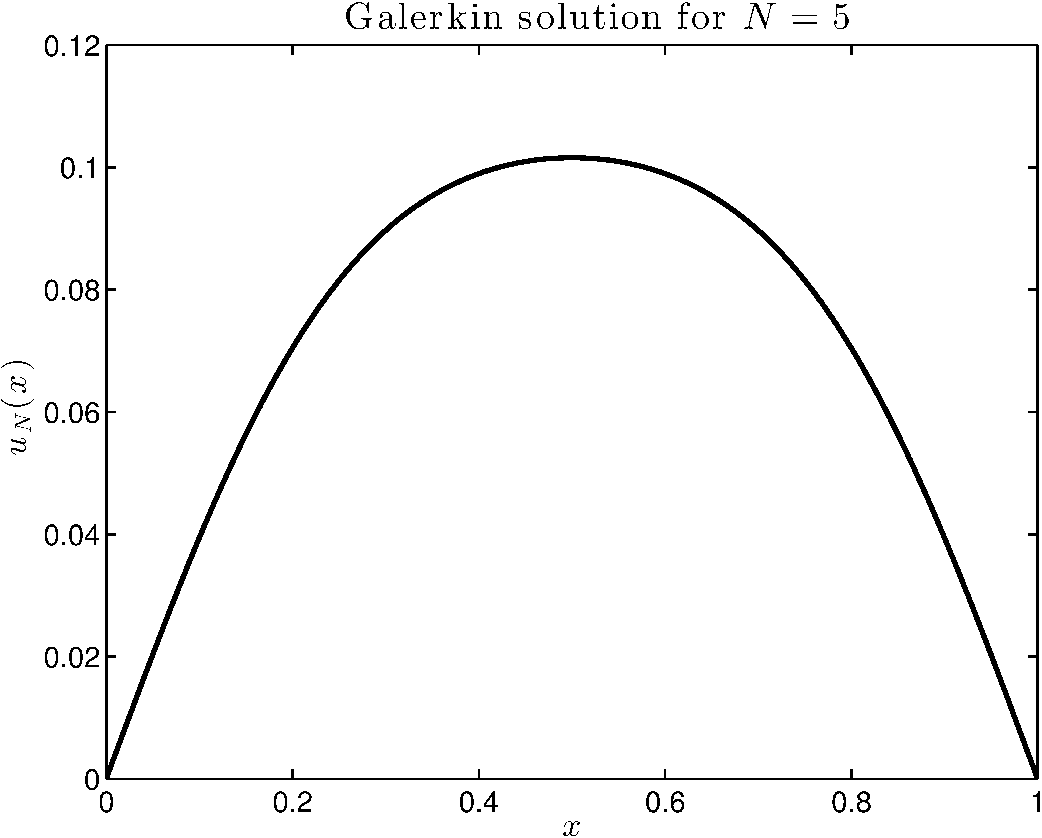
\includegraphics[scale=0.42]{delta_5}\quad
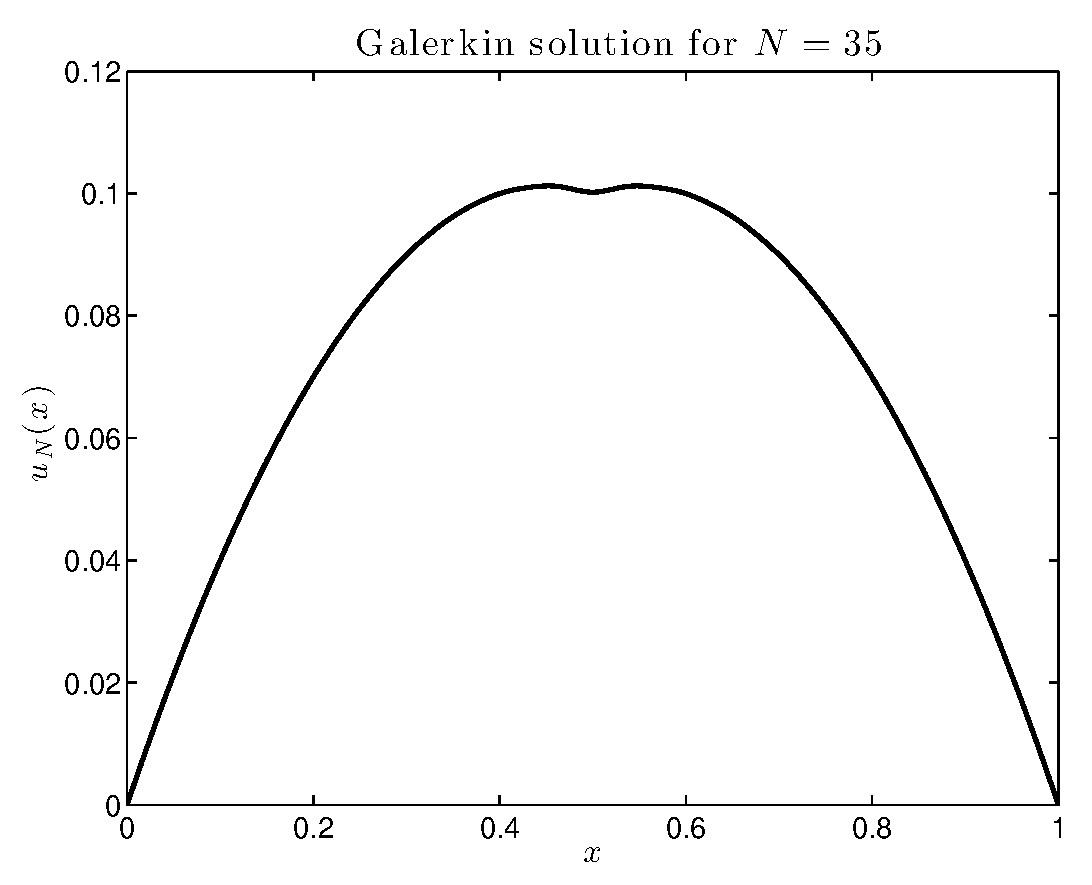
\includegraphics[scale=0.42]{delta_35}
\end{center}

\input delta_code
\end{solution}}{}

